% Data: research/n43/d18/parameter_landscape.json (schema version 1).
% Frontier window only: 0 <= q <= 17, 0 <= E_A = W_A <= 35.
% Inclusive JSON ranges become rectangles covering their integer cells.
\begin{figure}[htbp]
	\centering
	\begingroup
	\definecolor{landscape0}{HTML}{F7FBFF}
	\definecolor{landscape1}{HTML}{DEEBF7}
	\definecolor{landscape2}{HTML}{C6DBEF}
	\definecolor{landscape3}{HTML}{9ECAE1}
	\definecolor{landscape4}{HTML}{6BAED6}
	\definecolor{landscape5}{HTML}{4292C6}
	\definecolor{landscape6}{HTML}{2171B5}
	\definecolor{landscape7}{HTML}{08519C}
	\definecolor{landscape8}{HTML}{08306B}
	\begin{minipage}[t]{0.49\linewidth}
		\centering
		\textbf{(a) min-degree of forced $I_4 \subset A$}\par\smallskip
		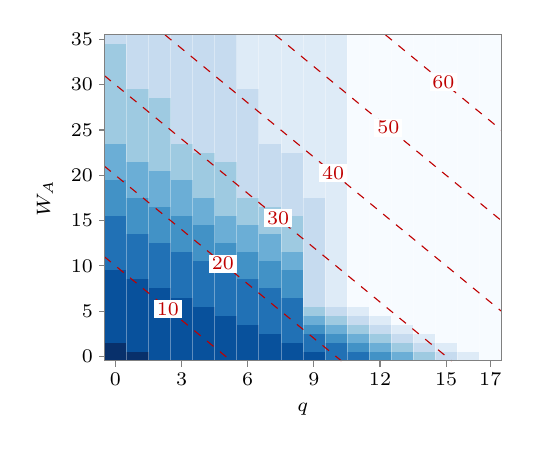
\begin{tikzpicture}[x=0.28cm, y=0.115cm, font=\scriptsize]
			% Entries are q / first excess / last excess / lower bound.
			\foreach \q/\lo/\hi/\value in {
					0/0/1/8,
					0/2/9/7,
					0/10/15/6,
					0/16/19/5,
					0/20/23/4,
					0/24/34/3,
					0/35/35/2,
					1/0/0/8,
					1/1/8/7,
					1/9/13/6,
					1/14/17/5,
					1/18/21/4,
					1/22/29/3,
					1/30/35/2,
					2/0/7/7,
					2/8/12/6,
					2/13/16/5,
					2/17/20/4,
					2/21/28/3,
					2/29/35/2,
					3/0/6/7,
					3/7/11/6,
					3/12/15/5,
					3/16/19/4,
					3/20/23/3,
					3/24/35/2,
					4/0/5/7,
					4/6/10/6,
					4/11/14/5,
					4/15/17/4,
					4/18/22/3,
					4/23/35/2,
					5/0/4/7,
					5/5/9/6,
					5/10/12/5,
					5/13/15/4,
					5/16/21/3,
					5/22/35/2,
					6/0/3/7,
					6/4/8/6,
					6/9/11/5,
					6/12/14/4,
					6/15/17/3,
					6/18/29/2,
					6/30/35/1,
					7/0/2/7,
					7/3/7/6,
					7/8/10/5,
					7/11/13/4,
					7/14/16/3,
					7/17/23/2,
					7/24/35/1,
					8/0/1/7,
					8/2/6/6,
					8/7/9/5,
					8/10/11/4,
					8/12/15/3,
					8/16/22/2,
					8/23/35/1,
					9/0/0/7,
					9/1/2/6,
					9/3/3/5,
					9/4/4/4,
					9/5/5/3,
					9/6/17/2,
					9/18/35/1,
					10/0/1/6,
					10/2/2/5,
					10/3/3/4,
					10/4/4/3,
					10/5/5/2,
					10/6/35/1,
					11/0/0/6,
					11/1/1/5,
					11/2/2/4,
					11/3/3/3,
					11/4/4/2,
					11/5/5/1,
					11/6/35/0,
					12/0/0/5,
					12/1/1/4,
					12/2/2/3,
					12/3/3/2,
					12/4/4/1,
					12/5/35/0,
					13/0/0/4,
					13/1/1/3,
					13/2/2/2,
					13/3/3/1,
					13/4/35/0,
					14/0/0/3,
					14/1/1/2,
					14/2/2/1,
					14/3/35/0,
					15/0/0/2,
					15/1/1/1,
					15/2/35/0,
					16/0/0/1,
					16/1/35/0,
					17/0/35/0
				} {
					\pgfmathtruncatemacro{\shade}{\value}
					\fill[fill=landscape\shade] (\q,\lo) rectangle ({\q+1},{\hi+1});
				}
			\foreach \q in {1,...,17}
			\draw[white, opacity=0.35, very thin] (\q,0) -- (\q,36);
			% Cell centers are (q+0.5,W_A+0.5), so 2X+Y = (x-136)+1.5.
			\foreach \level in {10,20,...,60} {
					\pgfmathsetmacro{\leftq}{max(0,(\level-34.5)/2)}
					\pgfmathsetmacro{\rightq}{min(18,(\level+1.5)/2)}
					\draw[red!75!black, dashed, thin]
					(\leftq,{\level+1.5-2*\leftq}) --
					(\rightq,{\level+1.5-2*\rightq})
					node[midway, fill=white, inner sep=1pt] {$\level$};
				}
			\draw[black!50, thin] (0,0) rectangle (18,36);
			\foreach \q in {0,3,6,9,12,15,17} {
					\draw[black!50] ({\q+0.5},0) -- ++(0,-0.7);
					\node[below, inner sep=2pt] at ({\q+0.5},-0.7) {$\q$};
				}
			\foreach \excess in {0,5,10,15,20,25,30,35} {
					\draw[black!50] (0,{\excess+0.5}) -- ++(-0.25,0);
					\node[left, inner sep=2pt] at (-0.25,{\excess+0.5}) {$\excess$};
				}
			\node[below] at (9,-3.6) {$q$};
			\node[rotate=90] at (-2.7,18) {$W_A$};
		\end{tikzpicture}\par\smallskip
		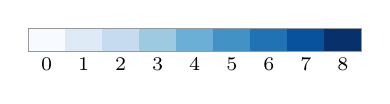
\begin{tikzpicture}[x=0.47cm, y=0.3cm, font=\scriptsize]
			\foreach \value in {0,1,2,3,4,5,6,7,8} {
					\fill[fill=landscape\value] (\value,0) rectangle ++(1,1);
					\node[below, inner sep=2pt] at ({\value+0.5},0) {$\value$};
				}
			\draw[black!40, thin] (0,0) rectangle (9,1);
		\end{tikzpicture}
	\end{minipage}
	\hfill
	\begin{minipage}[t]{0.49\linewidth}
		\centering
		\textbf{(b) Minimum column size}\par\smallskip
		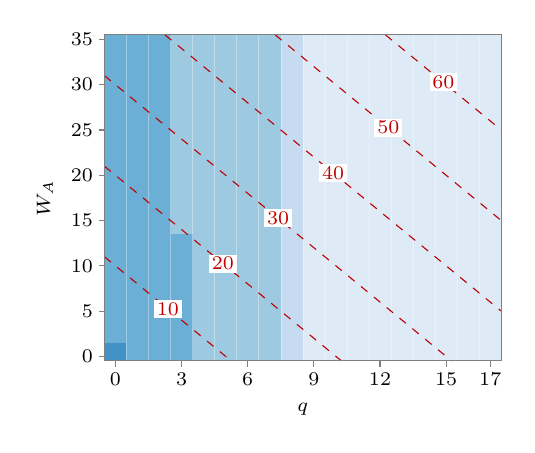
\begin{tikzpicture}[x=0.28cm, y=0.115cm, font=\scriptsize]
			% Entries are q / first excess / last excess / lower bound.
			\foreach \q/\lo/\hi/\value in {
					0/0/1/5,
					0/2/35/4,
					1/0/35/4,
					2/0/35/4,
					3/0/13/4,
					3/14/35/3,
					4/0/35/3,
					5/0/35/3,
					6/0/35/3,
					7/0/35/3,
					8/0/35/2,
					9/0/35/1,
					10/0/35/1,
					11/0/35/1,
					12/0/35/1,
					13/0/35/1,
					14/0/35/1,
					15/0/35/1,
					16/0/35/1,
					17/0/35/1
				} {
					\pgfmathtruncatemacro{\shade}{\value}
					\fill[fill=landscape\shade] (\q,\lo) rectangle ({\q+1},{\hi+1});
				}
			\foreach \q in {1,...,17}
			\draw[white, opacity=0.35, very thin] (\q,0) -- (\q,36);
			% Cell centers are (q+0.5,W_A+0.5), so 2X+Y = (x-136)+1.5.
			\foreach \level in {10,20,...,60} {
					\pgfmathsetmacro{\leftq}{max(0,(\level-34.5)/2)}
					\pgfmathsetmacro{\rightq}{min(18,(\level+1.5)/2)}
					\draw[red!75!black, dashed, thin]
					(\leftq,{\level+1.5-2*\leftq}) --
					(\rightq,{\level+1.5-2*\rightq})
					node[midway, fill=white, inner sep=1pt] {$\level$};
				}
			\draw[black!50, thin] (0,0) rectangle (18,36);
			\foreach \q in {0,3,6,9,12,15,17} {
					\draw[black!50] ({\q+0.5},0) -- ++(0,-0.7);
					\node[below, inner sep=2pt] at ({\q+0.5},-0.7) {$\q$};
				}
			\foreach \excess in {0,5,10,15,20,25,30,35} {
					\draw[black!50] (0,{\excess+0.5}) -- ++(-0.25,0);
					\node[left, inner sep=2pt] at (-0.25,{\excess+0.5}) {$\excess$};
				}
			\node[below] at (9,-3.6) {$q$};
			\node[rotate=90] at (-2.7,18) {$W_A$};
		\end{tikzpicture}\par\smallskip
		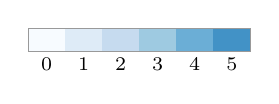
\begin{tikzpicture}[x=0.47cm, y=0.3cm, font=\scriptsize]
			\foreach \value in {0,1,2,3,4,5} {
					\fill[fill=landscape\value] (\value,0) rectangle ++(1,1);
					\node[below, inner sep=2pt] at ({\value+0.5},0) {$\value$};
				}
			\draw[black!40, thin] (0,0) rectangle (6,1);
		\end{tikzpicture}
	\end{minipage}
	\endgroup
	\caption{Each cell represents one integer pair $(q,W_A)$.
		In (a), the color corresponds to the interior min-degree of a forced independent set $I_4 \subseteq A$.
		The color zero indicates that no $I_4$ can be forced in $A$.
		In (b), the color $c$ guarantees $|C_w|\ge c$ for every $w\in B$.
		In both panels, dashed red contours are labeled by $x-136=2q+W_A$
		in increments of $10$, with integer parameter values located at cell centers.}
	\label{fig:parameter-landscape}
\end{figure}
